\documentclass[aps,prb,floatfix,amsmath,amssymb,amsfonts,10pt,floatfix,longbibliography]{revtex4-1}
\usepackage{amsmath,amsfonts,amssymb}
\usepackage{graphicx}
\usepackage{color}
\usepackage{subfigure}
\usepackage{bm}
\usepackage[colorlinks=true,
            linkcolor=blue,
            urlcolor=blue,
            citecolor=blue,
            unicode,
            pdfencoding=auto]{hyperref}

\begin{document}

\title{Learning Quantum Emergence with Artificial Intelligence}
\author{Paul Ginsparg}  %3,4,7
\author{Eun-Ah Kim}
\author{Roger Melko}
\author{Lei Wang}

\date{Today}
\begin{abstract}
Abstract here.
\end{abstract}
\maketitle


\tableofcontents
\newpage



\section{Introduction: Why AI for quantum emergence.}

(Lei: question to be addressed: why now ? why not 20 years ago ? 
abundance of data  -- but more importantly GPUs made it possible to train quickly enough and repeat to develop optimal heuristics for initialization and choice of non-linearities [relu]
latest development in AI (machine, software, techniques)
what do we expect from AI for quantum emergence: new discoveries in material, new physics, boost of existing techniques... 
) 

As significant advances in artificial intelligence (AI) capabilities, specifically in the area of machine learning, penetrate our everyday lives, similar methodologies have been increasingly adopted for use in scientific research \cite{Zdeborova2017}. The early adopters have been fields with data driven challenges such as astronomy, particle physics experiments, and genomics, to name a few. The use of machine learning in these fields has typically been to automatically process large amounts of data to suppress noise and highlight the signal of researchers' interest. [A bit more concrete description and reference?]

The rapid growth in use of %AI or
machine learning techniques
%\footnote{Loosely defined, AI is a broader class of computational scheme that includes machine learning. (Roger or Lei: more clarification.)}
%(PG -- yes, machine learning is a proper subset of AI, which is in turn a proper subset of theoretical computer science. If no AI methodologies other than machine learning are considered here, probably better to restrict to ML from outset)
in the study of quantum condensed matter over the last three years has 
been driven by two basic needs.
The first involves the underlying challenge of understanding complex quantum matter.
At a fundamental level, the purpose of studying quantum matter is to {\it understand essential phenomena\/} and the success of such understanding is reflected in the degree of knowledge compression\cite{kivelson-complexity}. A successful understanding of complex reality in the experimental or computational data of complex phase diagrams, or in many-body wave functions, amounts to a compression of that complexity in terms of simple principles such as entropy, electron-phonon coupling, topological invariants, and Fermi statistics. A test of the effectiveness of the compression is whether key features of the complex reality can be reconstructed and predicted starting from these simple principles.
For complex quantum matter, however, it is challenging to traverse either of the two paths depicted by arrows in Fig.~\ref{fig:learning}(a). It is then tantalizing to note that Machine learning tools specifically address these processes, under the terminology of {\it regression\/} and {\it classification\/} for the knowledge compression, and {\it generative modeling\/} for construction of key features. [learning representation (in latent space) for knowledge compression] Moreover, going back and forth is dubbed {\it hypothesis testing}.
Researchers have been naturally using the simplest versions of these tools when they plot and fit  data to a curve (Fig.~\ref{fig:learning}(b)), or partition phase space into different phases (Fig.~\ref{fig:learning}(c)). Finding a faithful representation of data in terms of a line with a linear fit, as in Fig.~\ref{fig:learning}(b), can both reveal a simple underlying principle and provide a compact representation to make the data easier to remember or reconstruct.  Similarly, grouping regions of phase space into different phase categories as in Fig.~\ref{fig:learning}(b) provides predictive power on a complex problem: the labelled phase characterizes what will result in the next experiment conducted under the conditions specified in that region of the phase diagram. Machine Learning tools can thereby play a natural role in our learning about quantum emergence. 

A second need arises from explosion in the volume of data. 
The famous macroscopic tunneling conductance measurement on Pb/MnO/Mg junction\cite{Giaever1962} offered confidence in the Bardeen-Cooper-Schrieffer theory of superconductivity because every detail of the measured curve (one-dimensional data) could be compared with the calculated density of state as a function of energy $N(E)$.
We do not, however, have the same means to understand the spatially resolved local density of state $N(\vec{r},E)$ measured by spectroscopic imaging scanning tunneling microscopy with atomic resolution, when $N(\vec{r},E)$ reveals rich and intricate spatial structure. Data-driven challenges have also become bottlenecks in analysis of classic reciprocal space probes: X-ray scattering and neutron scattering. 
In the days of point detectors, the bottleneck in scientific progress had been the sparse coverage of the reciprocal space. Now high-energy X-rays combined with area detectors at facilities such as Cornell High Energy Synchrotron Source provide comprehensive datasets, and new neutron sources equipped with large area detectors such as the Spallation Neutron Source (SNS) at Oak Ridge National Lab~\cite{SNS}, offer dense $(\vec{k},\omega)$ space data sets, and a key obstacle to discovery has become efficient analysis of the data~\cite{Miller2009,Stone2014-SNS}. 


%\item Why AI for quantum matter research? 

\begin{figure}[h]
\centering
\subfigure[]{
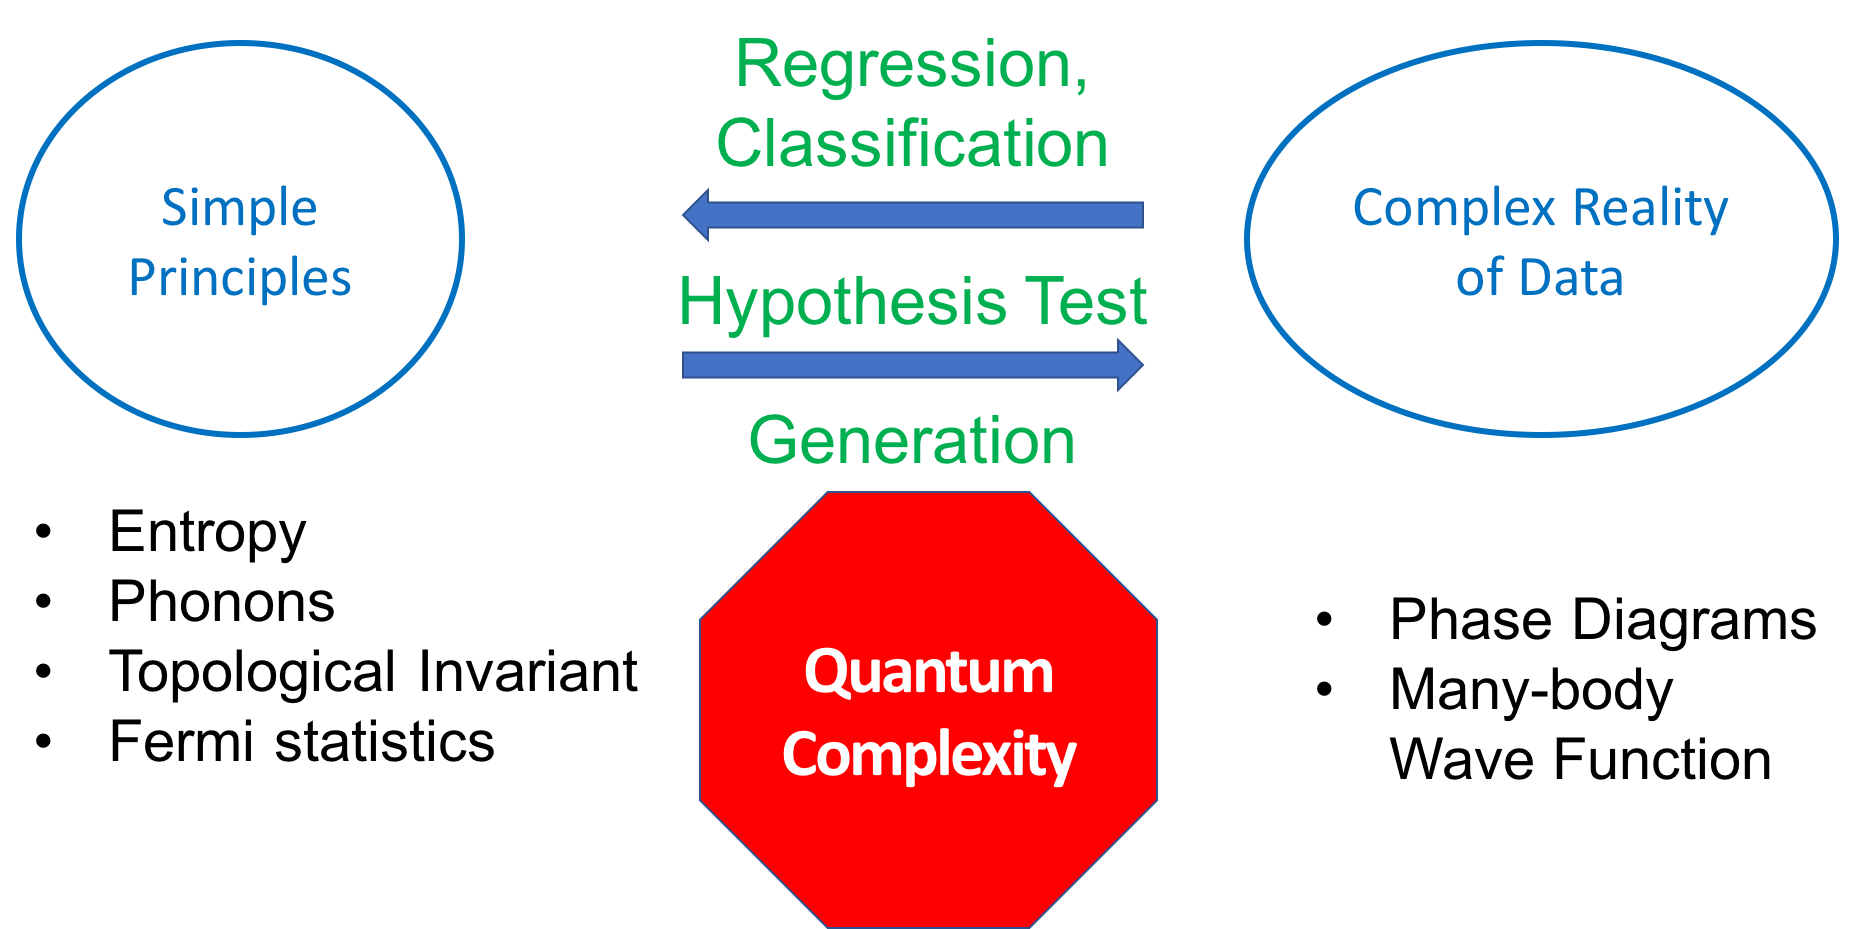
\includegraphics[width=.4\textwidth]{Figures/complexity.png}
}
\subfigure[]{
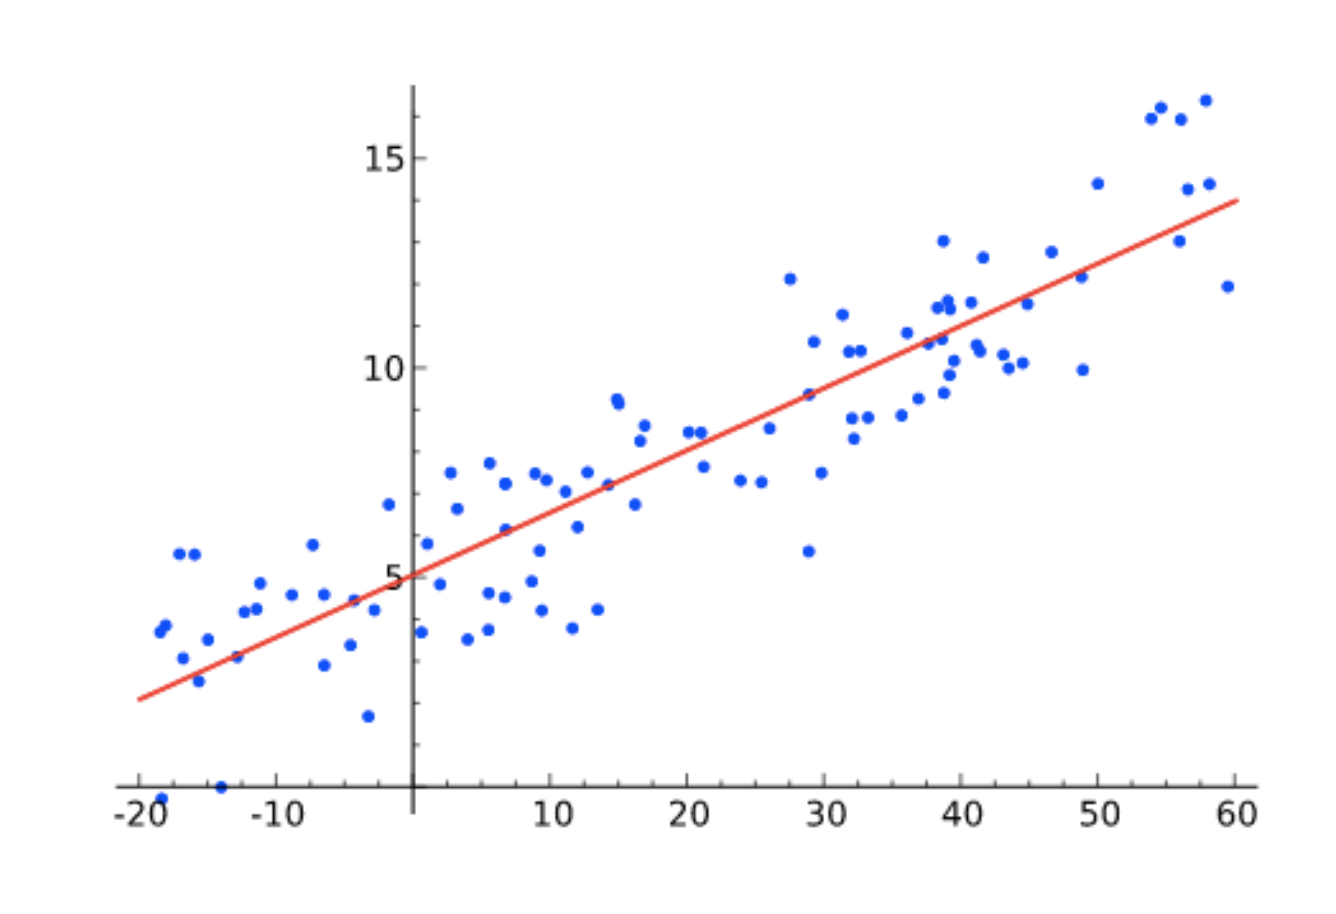
\includegraphics[width=.3\textwidth]{Figures/linear.png}
}
\quad
\subfigure[]{
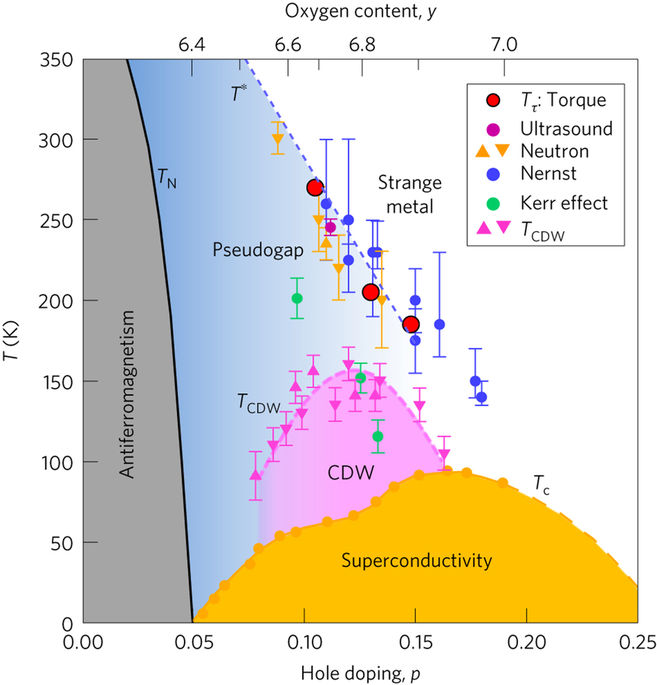
\includegraphics[width=.3\textwidth]{Figures/YBCO-PD-nphys4205-f3.jpg}
}
\caption{\label{fig:learning}
The understanding we seek from experimental and computational data requires regression. Learning a function (trend) from data (b) and classifying data into different phases (c) are both forms of regression. (b)XXX. (c)An experimental phase diagram of high T$_c$ superconductor YBCO.\cite{Sato2017}}
\end{figure}

Since the computational principle of machine learning is to develop a task specific intelligent machine, there is a great diversity in the approaches even within application to quantum matter.
The field is rapidly developing, so any attempt at comprehensive review will be soon dated. We will instead restrict to applications of machine learning involving artificial neural networks that illustarate the three modes highlighted in Fig.~\ref{fig:learning}: classification, generative modeling, and hypothesis testing.

Section~\ref{sec:ML} will present a pragmatic review of machine learning strategy using artificial neural networks (in short: deep learning).
Section~\ref{sec:phase} will review how the problem of obtaining phase diagrams have been efficiently treated as a problem of classification. Section~\ref{sec:WF} will review how the problem of expressing competitive (i.e, candidate ground state) many-body quantum states have been tackled as a problem of generative modeling. Section~\ref{sec:data} will discuss how the analysis of big experimental data can be treated as a problem of hypothesis testing. As the subject area is rapidly developing and too young to have a conclusion, we will close the review by discussing key open issues and the topics that we did not have space to do justice by way of conclusion. 

\section{The Machine Learning Strategy with Artificial Neural Network}
\label{sec:ML}

(Lei, Introduce landscapes of modern ML study: goal and tasks. Briefly introduce a few key techniques: ANN...)
The goal of machine learning is to identify regularities in data, and make use of them for predictions on unseen data. %Machine learning tasks tries to either discriminate input data or generate new data according to the learn probability distribution. 

\begin{enumerate}


\item (Paul) The Machine Learning strategy for complex computational problems is fundamentally different from that of traditional computational strategy. Fig.~\ref{fig:complex}. {\color{blue}[Ref]} 

[ok, note that i've started to clean this up in a separate file -- will insert]

\begin{figure}[h]
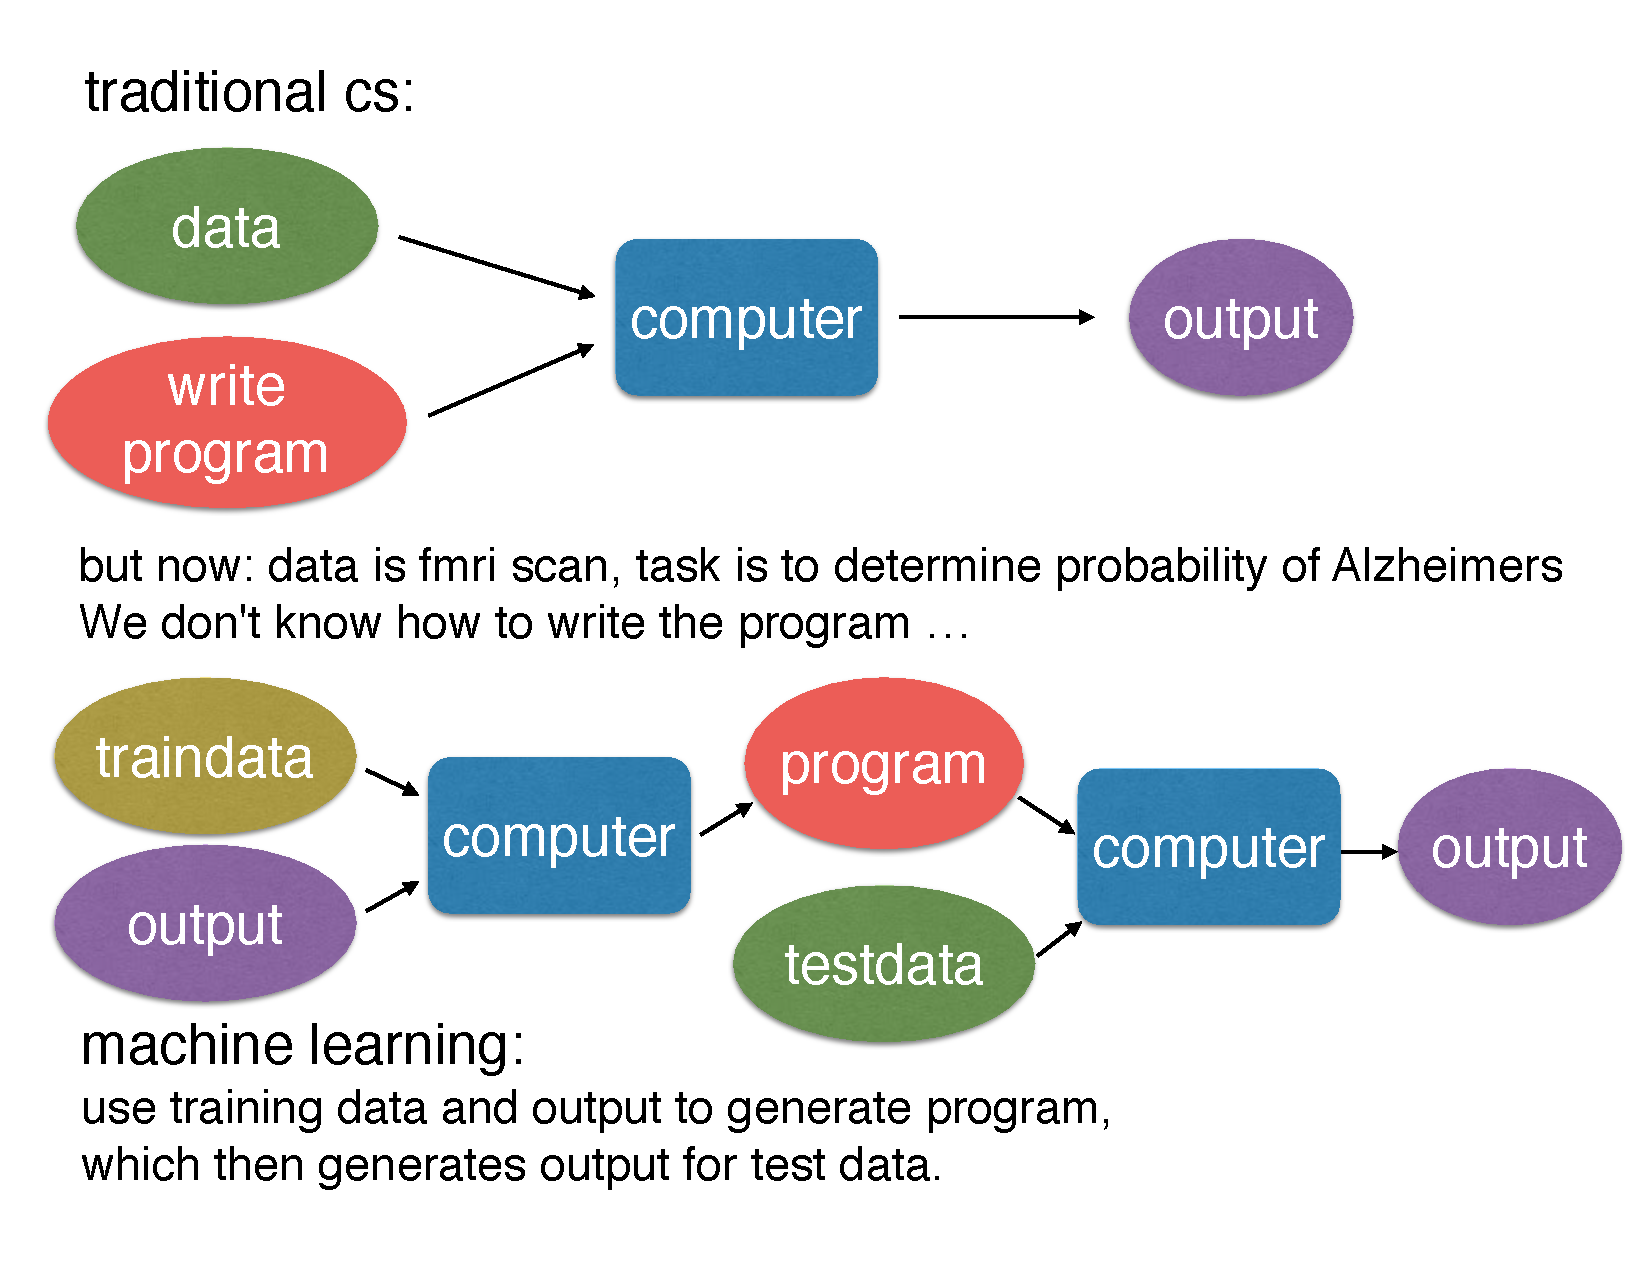
\includegraphics[width=.4\textwidth]{Figures/CS-modes-flow.pdf}
\caption{\label{fig:complex}
Machine learning strategy to solving complex problems.}
\end{figure}


\item (Paul) Perceptron and multi-layer perceptron. How hidden layer and non-linearity enable classification of data in high dimension. See Fig.~\ref{fig:non-linearity}. 
\begin{enumerate}
	\item Representing a function and classifying data are two faces of the same coin.
	\item A single (wide enough) hidden layer is sufficient to represent any function. {\color{blue}[Somewhat rigorous discussion with reference here.]}
	\begin{figure}[h]
	\centering
	\subfigure[]{
	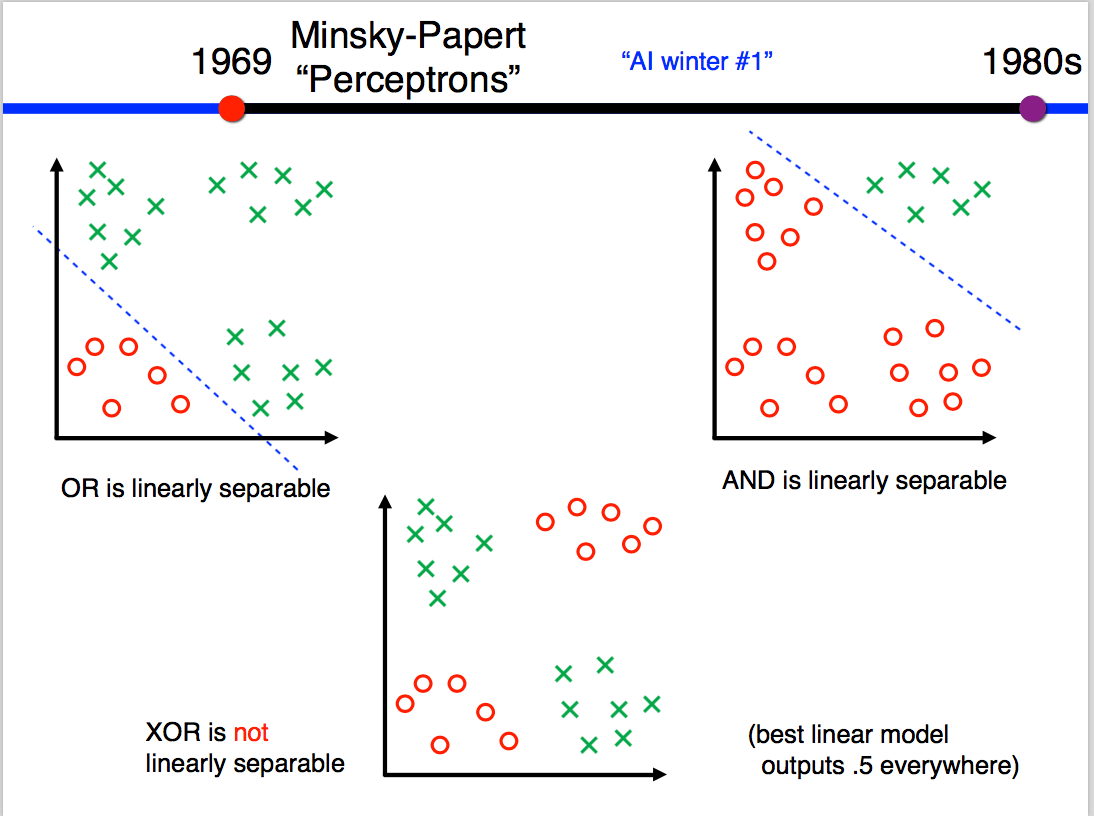
\includegraphics[width=.3\textwidth]{Figures/hidden-layer-0.png}
	}
	\hfill
	\subfigure[]{
	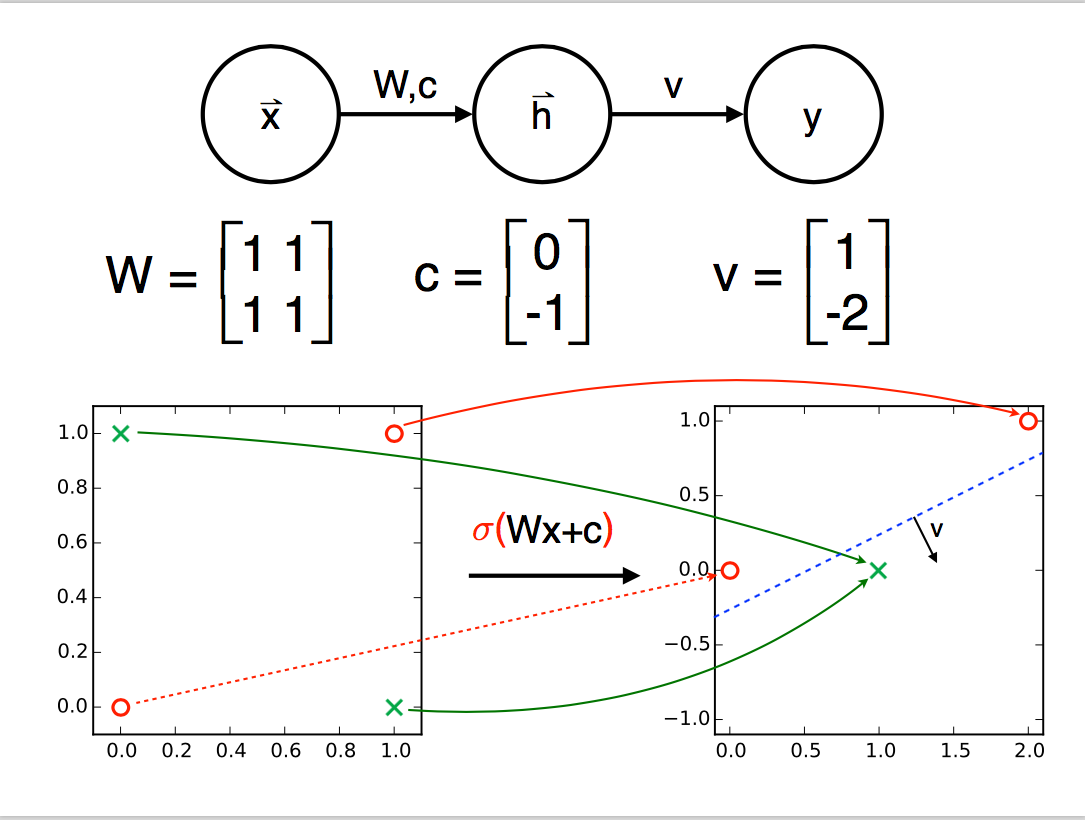
\includegraphics[width=.3\textwidth]{Figures/hidden-layer-1.png}
	}
	\hfill
	\subfigure[]{
	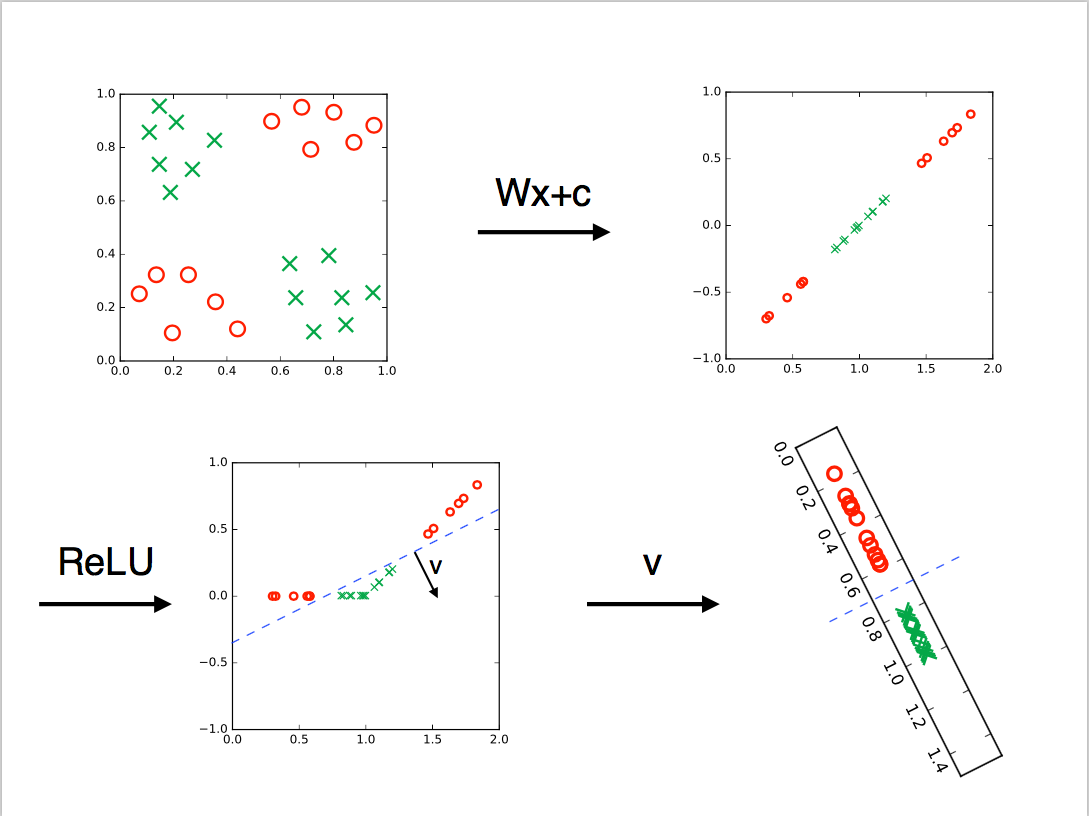
\includegraphics[width=.3\textwidth]{Figures/hidden-layer-2.png}
	}
	\caption{\label{fig:non-linearity} The benefit of non-linearity that comes with the firing function: versatility.}
	\end{figure}
	\item How multiple hidden layers combined with GPU led to the revolutionary progress.{\color{blue}[References to Hinton and ``successes".]}
\end{enumerate}

\begin{figure}[h]
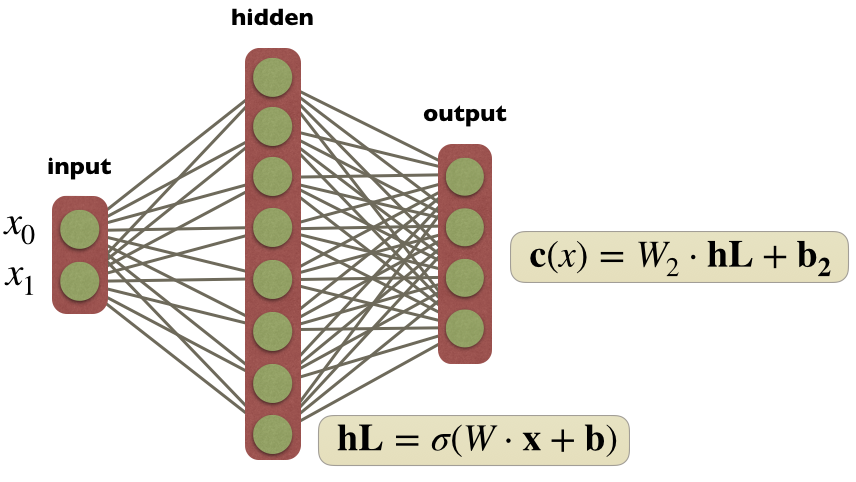
\includegraphics[width=.5\textwidth]{Figures/n2.png}
\qquad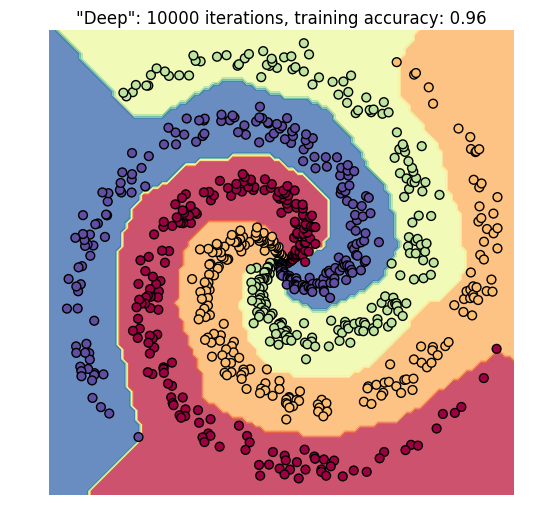
\includegraphics[width=.3\textwidth]{Figures/logistic2.png}
\caption{\label{fig:n2}
Simple classifier with single hidden layer to illustrate non-linear decision boundaries.}
\end{figure}



\item (Eun-Ah, How weights and biases guide the ANN's decision.) To see how ANN's decisions on given input are determined, it is illustrative to consider a setting that involves human decision making. Consider a child's decision upon dropping food. For an illustration purpose, we will model this decision making process using a fully connected feed-forward ANN with a single hidden layer .\cite{Nielson2013} He or she will take various inputs such as whether parents are watching, how long has it been since the food fell, whether it is sweet. Each of this input information in ANN is represented as a component of input vector $\vec{x}$. Different parts of the child's brain will weigh different input component with varying degree of importance. With ANN, we represent this by neuron-specific weight, i.e., neuron $i$ will put weight $w_{ij}$ on the input component $x_j$. (See Fig.~\ref{fig:decision} for illustration.) Finally, each input component will be biased in the decision one way or another, e.g., either to pick-up and eat the food or not. This neuron specific bias is $b_i$. Each neuron $i$ will fire when $w_{ij}x_j+b_i$ exceeds a threshold. This threshold is represented by the non-linear firing function such as rectified linear unit $\sigma(z)^{\rm ReLU}\equiv {\rm max}(0,z)$. Each neuron's firing gets collected with different weight $v_i$ by the output neuron which declares the decision $y$. This whole process is compactly captured as: 
\begin{equation}
   y(\vec{x})= \sigma \left(\vec{v}^T\cdot\sigma(\tilde{w}\cdot\vec{x}+\vec{b})\right).
\end{equation}
Notice that the critical step in making the output a non-linear function of the input $\vec{x}$ is the firing function associated with the hidden layer. Although the decision is a non-linear function, the complete specification of the weights $\tilde{w}$ and biases $\vec{b}$ uniquely determine the outcome for the given input. The training of the ANN is about guiding the ANN to find the the weights $\tilde{w}$ and biases $\vec{b}$ that lead to the desired decision by giving feedback on the output $y(\vec{x})$. For a supervised machine learning, the goal would be to minimize the difference between the actual output $y(\vec{x})$ and the desired output $a(\vec{x})$ that is measured through various cost functions $C[\tilde{w},\vec{b}]$. 


	\begin{figure}[h]
	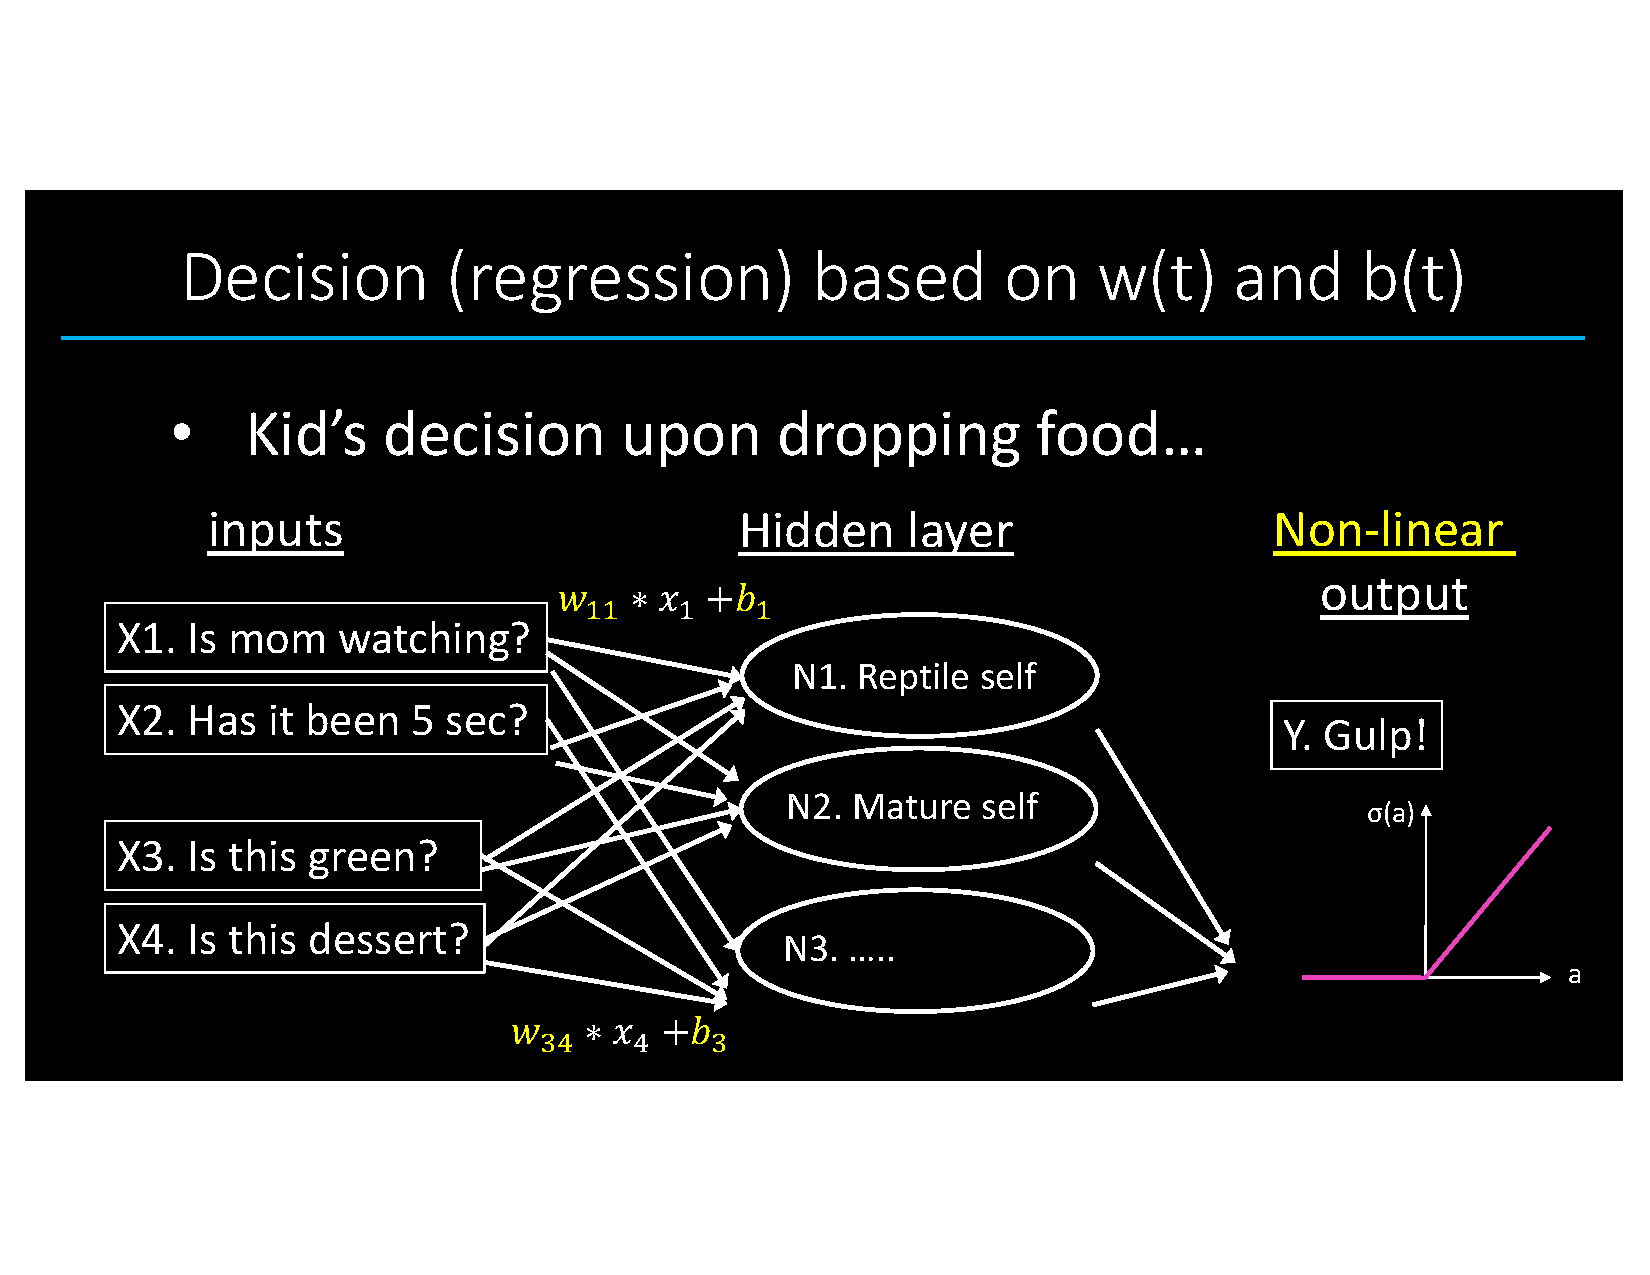
\includegraphics[width=.4\textwidth]{Figures/decision.pdf}
	\caption{\label{fig:decision}The weights $w_{ij}$ and biases $b_i$ associated with hidden layer neuron $i$ specify how the input component $x_j$ will be processed by the neuron $i$ to ultimately lead to a decision. }
	\end{figure}

\item (Paul) How to train ANN to make the correct decision using back propagation. Avoiding over-fitting.

\item (Roger)  Hopfield to RBM. 

	
\item (Lei) Architecture design of the neural networks by incorporating the inductive bias of the to be modelled distribution is is one of the most important issue in modern deep learning research. Appropriate inductive bias not only allows more parameter efficient description of the data, but also can reduce the difficulty in the optimization. The convolutional neural networks exploits the inductive bias of natural images which are related to the local and translational invariant features, and exhibits superior performance compared to the unstructured neural networks. When applying technology to the physics datasets, it is also crucial to incorporate inductive bias of the particular physical problems. 
	
\item Other Neural Networks: RNN, etc?

(Lei, High level view of the neural networks) Despite of the biological analog often been mentioned, the neural networks are can be better understood as an information processing device to a physicists. A neural network maps the input to the output signal through a deterministic or stochastic channel. This view point, demystifying the neural networks and puts them in the same category as other computational devices such as the tensor networks and the quantum circuits. %This perspective also strongly calls for an information perspective on the neural networks. 
  
\end{enumerate}  

\section{Phase Detection: Classification}
\label{sec:phase}
The basic idea of using machine learning for phase detection is to employ the ability of modern machine
learning techniques to classify, identify, or interpret massive data sets, to efficiently obtain the phase diagram\cite{Carrasquilla2017a}. 
Microscopic hamiltonians relevant for quantum matter  are not exactly solvable in general and hence their theoretical understanding require numerical simulations. Moreover, due to  the fact that the Hilbert space of quantum many-body system grows exponentially with the number of particles, simulations of some hamiltonians (i.e., models with the ``sign-problem'' [CITE]) would never converge at low temperature. Nevertheless much progress have been made with models that do not suffer from the ``sign-problem''  that are nevertheless quite rich \cite{Berg2012,Schattner2016a,Gerlach2017,Xu2017a,Lederer2017,Li2016,Li2017,Jiang2017}. Nevertheless it is often computationally costly to obtain the phase diagram even in this models. 

Conventionally, in order to obtain the phase diagram associated with a model one first defines a grid in the phase space and identify the phase of the model at each phase space point. This identification follows a two step process. The first step is to converge the simulation of the model at the phase space point. The second step is to evaluate the expectation value of the relevant operators, called estimators, that label the phases. The estimators are often physical observables that have traditionally played key roles in our understanding of quantum matter due to the fact that they can be experimentally measured. Among such are order parameters, superfluid density, specific heat. In Monte Carlo simulations which are among the most powerful approach to quantum many-body simulation, these estimators are obtained from the states sampled from the state space through stochastic importance sampling. The expectation value of the estimators are reached by averaging out the fluctuations in each sampling. Once the phase associated with a given phase space point is identified, the whole process is repeated at the next phase space point. 

The phase diagram acquisition becomes challenging when important new states of matter are impervious to the standard estimators. This is the case with the topologically ordered states\cite{Wen1990IJMPB} which can be detected using topological entanglement entropy\cite{Levin2006,Kitaev2006} that is prohibitively expensive and challenging to measure experimentally\cite{Islam2015}. This is also the case with all out-of-equilibrium eigenstate phases\cite{Huse13, PekkerHilbertGlass} in the context of many-body localization (MBL) \cite{Anderson58, Basko06, PalHuse,  OganesyanHuse,  AltmanVosk}. The phase diagram acquisition can also be challenging simply because simulations offer sparse information on the defining characteristic of a phase, as is the case for transport properties. 
Rigorous information on transport one can gain from simulations is limited because simulations yield imaginary time data, and the analytic continuation of imaginary time data to real time is numerically ill posed. Nevertheless, the imaginary time current-current correlation function must contain the nugget of the key information regarding transport. Indeed 
superfluid density can be rigorously obtained to signal superconductivity\cite{Scalapino1993} and even a “proxy” for the DC resistivity can be obtained to hint at non-Fermi liquid behavior\cite{Lederer2017}, all starting from current-current correlation function. 

In both of these challenging situations Machine Learning approaches have proven invaluable in enabling efficient acquisition of phase diagrams by recognizing phases in the midst of the statistical and quantum fluctuations as we will discuss below. 


\subsection{Supervised Learning}
In the supervised learning approach the ANN's are trained with the ``labeled data'' and then asked to classify new data into the classes associated with the labels. As the ANN has to find the characteristics it has come to identify with a specific label in a data set it has never seen before, the success of supervised learning depends on the diversity of the training set within each label. 
For the phase diagram acquisition supervised learning is typically implemented by using data from known asymptotic limits as labeled training set\cite{Carrasquilla2017, Zhang2017,Zhang2017a,Broecker2017,Broecker2017a,Schindler2017,Ohtsuki2016,Nieuwenburg2017}. Unlike the conventional approach which demands the effort of averaging out the fluctuations in the estimators at all points of the phase space, the supervised learning approach only requires efforts in training the ANN which depends on a diverse set of data at training points. Once an ANN is successfully trained, it rapidly classifies data from the rest of the phase space to reveal the phase boundaries as the region of the phase space where ANN is confused\cite{Nieuwenburg2017}.

For the supervised learning for phase detection to be successful the machine needs to be able to discover and learn the phase defining traits in the training data. In the image recognition challenges that have been driving the developments in supervised learning [CITE] the format of the data is fixed to be an optical image. In optical images an object is defined in terms of the shape of the boarder and the color distribution within the region inside the boarder. The successful use of convolutional filters combined with pooling layer for automated feature detection and data compression for the image recognition hinges on the fact that convolutional filters are well-suited for learning the boarders. 

Unlike optical images,  human engagement is inevitable with quantum many-body data since measurement is basis-dependent. Hence, even if one avoids any further pre-processing, there is human engagement in the choice of basis. For equilibrium symmetry breaking phases with a known order parameter the problem is classical in the order parameter basis. When the order parameter basis is also a natural basis for Monte Carlo, a standard feed-forward neural network can be trained to detect multiple types of order parameter directly from raw state configurations sampled with Monte Carlo as it was first demonstrated in
Ref.~\cite{Carrasquilla2017a}. In the traditional approach to a phase diagram acquisition using Monte Carlo, exponentially large state space is sampled through a stochastic importance sampling and then estimators for physical quantities are calculated from these samples to yield equilibrium expectation value of the estimator
(sanvik AIP conference proccedings 1297 (2010)).
In the supervised learning approach of Ref.~\cite{Carrasquilla2017a}, two different types of raw Monte Carlo configurations belonging to the magnetically ordered phase and the paramagnetic phase are accurately classified despite thermal fluctuation in each configurations, without the use of any estimator. Here configurations from different temperatures are given to the trained neural network (implemented with Tensor Flow (M. Abadi, et al., TensorFlow: Large-scale machine learning on heterogeneous systems (2015).
Software available from tensorflow.org.) at once and their classification boundary reveals the transition temperature. 

However states of modern interest such as topologically ordered state [CITE] and out-of-equilibrium state [CITE] cannot be identified by order parameters. It has been clear from early on that identification of even  symmetry breaking transitions from raw configurations is challenging when  the basis of Monte Carlo simulation is different from the order parameter as in the determinant Monte Carlo simulation of fermionic problems. [CITE]. Under such circumstances the full complexity of quantum matter requires approaches that can pass relevant information to the fully-connected neural network. 

For out-of-equilibrium many-body localized phases, entanglement spectra. 
Entanglement spectra\cite{Li2008} encode key information that defines phases that evade the traditional
notion of order parameter. In systems with translational (rotational) symmetry, the distribution of
entanglement spectra as a function of (angular) momentum has revealed qualitatively distinct characteristics
for topological phases\cite{Li2008,Thomale2010,Qi2012}. However, quenched disorder negates this proven scheme. In Refs. ~\cite{Nieuwenburg2017,Schindler2017,Venderley2017} feed-forward neural networks have successfully identified  many-body localized phases yielding out-of-equilibrium phase diagrams. 
In particular, Ref.~\cite{Venderley2017} demonstrated that neural network based approach can surpass existing manual approach in finding sharper phase boundary. 

Another physically motivated successful feature selection process is the quantum loop topography \cite{Zhang2017a,Zhang2017}: a procedure of constructing a multi-dimensional image from the ``sample'' Hamiltonian or wave function by evaluating two-point operators that form loops at independent Monte Carlo steps.
The loop configuration is guided by characteristic response for defining the phase, which is Hall conductivity for integer and fractional Chern Insulator\cite{Zhang2017a} and 
interlocking Wilson loops associated with spinon and vison in Z2 quantum spin liquid\cite{Zhang2017}. 
Refs.~\cite{Zhang2017a,Zhang2017} demonstrated the potential of quantum loop topography as an alternative to convolutional layer for passing relevant non-local information to the fully connected layer. 
  


({\it Support Vector Machines:})
Not all supervised learning methods use neural networks.  For example, classification studies can be performed using techniques such as support vector machines (SVMs), one of the most common tools for supervised learning.  SVMs have been successfully applied previously in interpretable discovery of order parameters in condensed matter systems.  

Linear support vector machines were first designed to perform binary classification with supervised learning, taking an input and predicting which of two labels the data is most likely to belong.  In this case SVMs attempt to simply find the hyper-surface which best separates the two classes.  Once this hyperplane (called a decision boundary) is found for a training set, it is used to make predictions on a test set.

Since many data sets may not have linear decision boundaries, SVMs are routinely extended to via the {\it kernel trick}, whereby the decision function is modified with some non-trivial choice of kernel.  
The kernel depends on the inner product of spin vectors like Eq.~XXX, but can otherwise have some freedom in definition.
They have the effect of mapping the data to a higher dimensional feature space, where linear separation may then be possible.   

It was shown by Ponte that the decision function can be interpreted as an order parameter of a condensed matter system.  For the simple case of an Ising model undergoing a PM to FM transition, a quadratic kernel is sufficient to have the decision function manifest $\langle m^2 \rangle$, the squared-magnetization order parameter.  This work has been extended recently to ...

Although not as scalable, SVMs offer an important advantage over other methods such as neural networks. The ability to use different kernels for classification tasks allows SVMs to find {\it interpretable} physical discriminators for different models, 
by relating the decision function to quantities such as conventional order parameters defined in condensed matter systems.
The ability of SVMs to find the mathematical structure of order parameters may have consequences for the study of spin liquids, which are often pragmatically defined as lacking any conventional order.  SVMs offer a systematic way to search for and exclude conventional long range order, where the complexity of the order parameter increases with the complexity of the kernel.


\subsection{Unsupervised Learning}

The vast majority of data in the world is presented to us unstructured and unlabelled.  The process of physical discovery often begins with such data; the goal of a physicist is to uncover the internal structure, and to eventually link it to fundamental models and theories of nature.  As a machine learning problem, unlabelled data presents us with a very different paradigm than the labelled data discussed in the last section.  Without labels, there are no correct or incorrect answers; in the absence of a teacher, the problem becomes {\it unsupervised}.  Algorithms must be designed to uncover and present interesting structure in data, based on their own devices.  The large number of possible ways to do this means that unsupervised learning has many facets.  

Here, we discuss two broad approaches to unsupervised learning for unlabelled data sets. The first is {\it clustering}, which aims to discover the inherent groupings in the data.  The second is {\it generative modelling}, which aims to learn an approximate probabilistic model that underlies the distribution of the data. One can then use the generative model to infer missing data or generate new data according to the learned probability distribution. 

\subsubsection{Clustering}

Imagine a set of measurements, raw and unprocessed, taken in different regions of a phase diagram.  The first question one may ask of this data set is how many phases are represented within.  This is an example of a situation where learning inherent groupings of the data points may help uncover common physical structure and correlations.  We begin with the idea of clustering, with the idea of mapping high-dimensional data to lower dimensions (typically two) in order to capture and visualize internal structure.

\item (Lei) Principal component analysis (PCA) is arguably the simplest dimension reduction technique. PCA projects the original data into a linear subspace which keeps most of the variation of the original data. For example, the PCA analysis of the Ising configuration collected at various temperatures shows that the greatest variation is in the magnetization, which corresponds to the first principal component. When project to the low dimensional space spanned by the first few principal components, human or clustering algorithms can identify clusters which corresponding to different phases in an unsupervised fashion. Besides being used for studying phase transitions, PCA was also used to extract low dimensional representation of atoms for identifying clustering~\cite{Atom2Vec2018}. 

%ICA
A related dimension reduction technique, the Independent component analysis (ICA), seeks for a subspace where each component are mutually independent in the information sense. A typical application is the cocktail party problem, where one aims at isolate the speech of each single person from  mixed signals picked by multiple microphones. 
Both PCA and ICA are linear perform linear transformations. This limits their application to cases where the relevant feature is nonlinear function of the original data. 

\item (Roger) t-SNE on Ising model \cite{Carrasquilla2017a}

Another modern dimension reduction technique is the t-distributed stochastic neighbor embedding (t-SNE).  It was developed by van der Maaten and Hinton as an attempt to generalize linear frameworks, like PCA, to be sensitive to non-linear structure in data. Like PCA, the typical t-SNE learning problem is unsupervised, in that it learns structure from the data itself without the use of predetermined classifications.  Additionally, t-SNE is able to embed higher-dimensional data into lower dimensions (typically two), 
so that data points close to each other in the original space are also positioned close to each other in the embedded low-dimensional space.  Thus, correlations between data points can be manifest as easy-to-visualize clusters, suitable for quickly exploring hidden structure in large, unlabelled data sets.


\item (Roger/Lei) t-SNE and auto-encoder on half-filled Hubbard model \cite{Chng2018}
Variational auto-encoders can be regarded as nonlinear generalizations of the PCA, in which the latent space encodes the learned feature. 

Clearly, such a framework does not provide the same quantitive understanding as a direct
Monte Carlo measurement of the order parameter, which sits on a solid bedrock of decades
of statistical mechanics theory.



\subsubsection{Generative Modelling}
\label{sec:WF}
%\subsection{New approaches to VMC}
\begin{enumerate}
\item (Roger) Goals of generative modelling: state reconstruction
\item (Roger) Hopfield networks and RBMs.
\item (Roger) 2D Ising model
\item (Roger) Experimental prospects

\item (Lei) Generative models aim at describing the data generative process via modeling the joint probability of high-dimensional data. Thus they capture all patterns that are present in the data other than merely the conditional mapping from data to particular label. Latest development of generative models. Deep generative models is one of the frontiers of deep learning research. Major modern generative models include the variational autoencoders, generative adversarial networks, autoregressive networks and normalizing flows. Application of them spans from unsupervised learning of phase transition, to quantum state tomography, and to holographic normalization group. One of the most significant feature over the energy-based model is that they all allows direct sample generative. Moreover, some of the models even allow explicit and tractable computation of likelihoods, which is an important feature in quantitative study of problems in physics. 


\section{Theoretical Insight from Experimental Data}
\label{sec:data}
%(Lei: So, this section is for machine learning experimental data ? Maybe an more informative section title ?)
Besides learning from the synthetic data out of computer simulations, it is even more exciting to directly apply machine learning techniques to real experimental data. With the aid of machine intelligence, one can test theoretical scenarios, develop physical understandings, and even make scientific discoveries. 

%The essentials of the scientific discovery process have remained largely unchanged for millennia: systematic human observation of natural phenomena is used to form hypotheses that, when validated through experimentation, are generalized into established scientific theory. 
Today we face many major scientific challenges driven by big experimental data. This is because automated scientific instrumentation and large-scale data acquisition have revolutionized empirical science by generating data sets of such volume and complexity as to defy human analysis. A promising direction would be to use machine learning to interface human intellect with the 
enormous data sets laden with noise and enable scientific discovery. 
Another challenge coming with the rapid progress in quantum computation architectures is XXX ( tomography, error correction) 

%Efforts in such synergy are at their infancy. Yet since these approaches are versatile, we review established proof-of-principles. 
%\item (Eun-Ah) Explosion in the volume of experimental data. Position space visualization of spectroscopy and momentum space visualization of spectroscopy
%\item (Eun-Ah)Complexity of the problem of quantum emergence requiring new criteria for understanding, or knowledge compression/regression. Constraints from fundamental laws of physics.
%In the long term, it would be ideal to discover correct theory from large data through unsupervised learning. However, unsupervised learning is still very much under development. 
%The immediate goals are to accomplish parts of the long term goal by 1) testing large data against a finite set of hypothesis using supervised learning or 2) XXX [to be aligned with tomography].

%\item (Eun-Ah) Immediate goals:
%    \begin{enumerate}
%        \item Discerning different theoretical hypothesis.
%        \item Exhaustive processing of large-dimensional data.
%    \end{enumerate}
%\item (Eun-Ah) Longer term goals: Discovering the correct theory from large data.




\subsection{(Eun-Ah) Proof of principle with the STM data (to be polished and shortened)}
 Ref.~\cite{Zhang2018} have developed a three stage supervised learning protocol for discerning data against different theoretical hypothesis.
Stage
1 of the protocol is to 
generate a training set that
is labeled with the ideal theoretical
hypotheses but simulated with real-
life mimicking noise. Stage 2 is to  build and train 
ANN’s with the training data.
Whether the networks  can be trained with the
training data will already be a nontrivial
exercise revealing whether different hypothesis
 can be distinguished
when scrambled with real-life level of
noise. 
Finally, Stage 3 is to test
experimental data on various
trained ANNs. Since the training of ANN's is a stochastic process, multiple ANN's trained simulatneously will generally have different weights and biases. By having different networks, one can assign error bars to the ANN output that categorizes experimental data (see \ref{fig:STM-results}(a)).

 

Historically, charge modulations have been associated with reciprocal space structure (Fermi surface nesting)\cite{gruner} (see Fig.\ref{fig:STM-problem}(b)). But
  strong Coulomb interaction between electrons promote the electrons to form position space structures (see Fig.\ref{fig:STM-problem}). 
 Hence being able to discern these two attributes can impact a fundamental understanding of charge modulations ubiquitously observed in modern EQMs \cite{Abbamonte2005,Ghiringhelli2012,Kogar2017,Zhang2016,Gerber2015,Bugaris2017,CoBaNi2As2} (see Fig.\ref{fig:STM-problem} for a typical data set a t the fixed energy). 
\cite{Robertson2006,DelMaestro2006}.Given this objective, Ref.~\cite{Zhang2018} chose  modulations with $Q_0=(0.23, 0.25, 0.27, 0.29)2\pi/a_0$ as hypothesis  for generating synthetic training data labeled with categories 1,2,3,4 respectively. These $Q_0$ were chosen based on the broad distribution of the Fourier transform of experimental data. Among these category 2 with $Q_0=0$ was the only commensurate category. 
 Ref.~\cite{Zhang2018} addressed the issue of bi- or uni-directionality by testing experimental data in two orientation and comparing the trained NN's confidence in each categories for the two orientations. 

The results of Ref.~\cite{Zhang2018} are striking. 3D data  of Z-map from underdoped cuprate high $T_c$ superconductor at hole-doping range $0.07<p<0.17$ were tested. Despite short correlation lengths and the related the lack of any sharp features in the  Fourier transforms of the image array, the NNs detected a remarkable universality and simplicity underlying the rich and complex data set presented:
(1) the NNs overwhelmingly favor category 2 ($Q_0=\frac{2\pi}{4a_0}$) and (2) the confidence is substantially higher in one direction over the other (see Fig.~\ref{fig:STM-results}(b)). These results point to 
a very specific ordered state with lattice-commensurate, 4a0 periodic, unidirectional, translational-symmetry breaking state. The fact that such state is recognized at all energies (Fig.~\ref{STM-problem}(c)) 
is providing first confirmation of the universal relevance of the theoretical prediction\cite{Zaanen1989,Loew1994, Vojta1999,White1998a,Capponi2002, Corboz2014,Fischer2014}  depicted in Fig.~\ref{fig:STM-problem}(c). 

Concurrently, a milestone for the quest of learning quantum emergence
has been achieved with the demonstration that ANN’s can process and identify specific broken symmetries of highly complex image-arrays from non-synthetic experimental EQM data, through an ANN-human coalition. Overall, these combined advances open the immediate and exciting prospect of additional ML-driven scientific discovery in EQM studies. 



\begin{figure}[t]
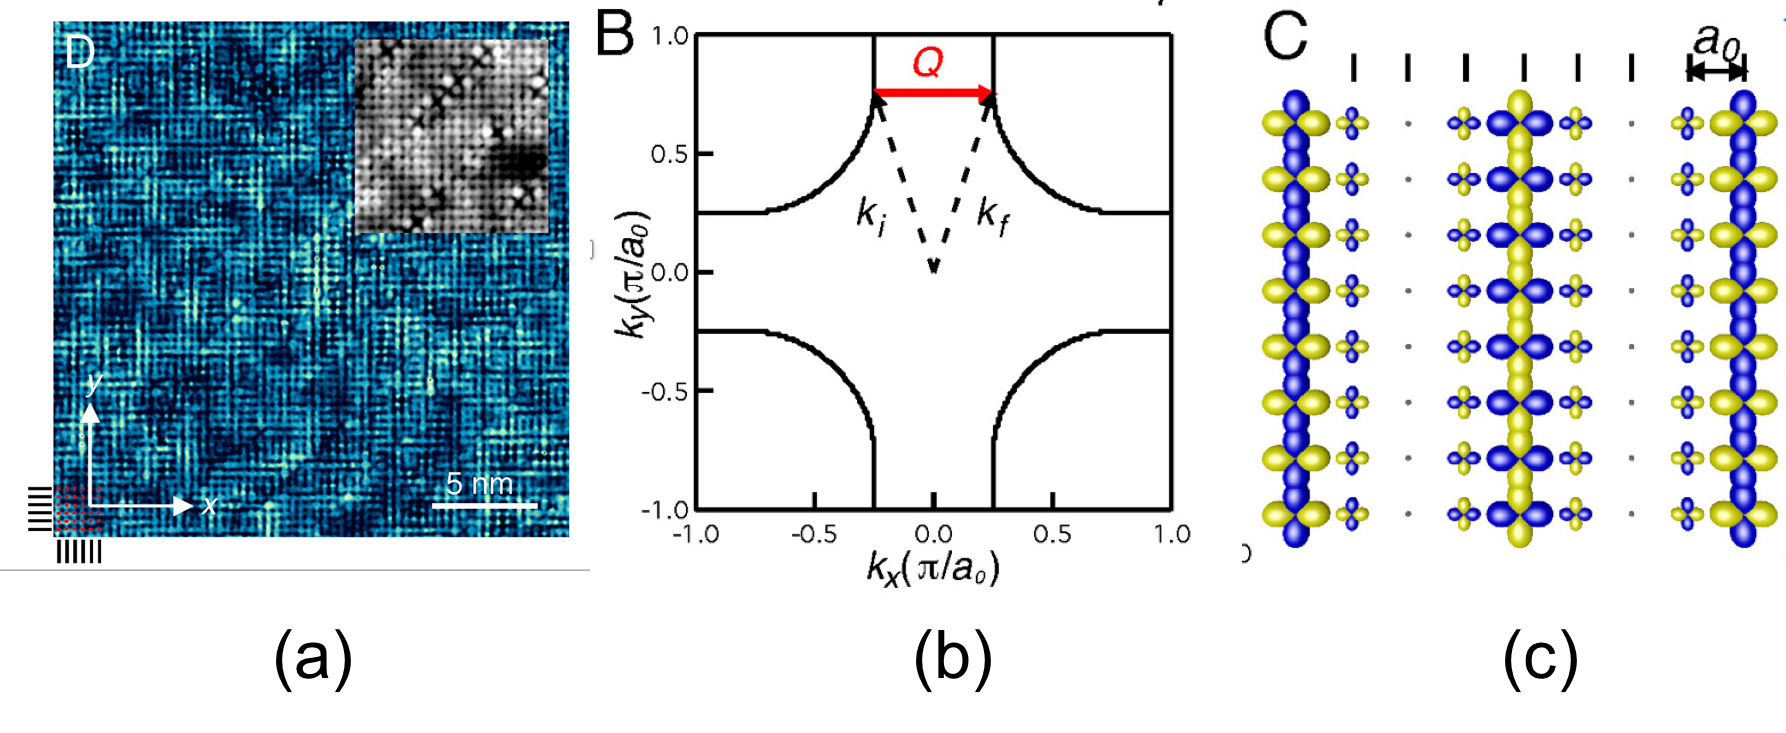
\includegraphics[width=\linewidth]{Figures/STM-problem.png} 
\caption{(a) Typical 24.4nmX24.4nm SISTM image of electronic structure  from the CuO$_2$ plane of Bi$_2$Sr$_2$CaCu$_2$O$_8$ with $p=0.08$ ($T_c=45K$) exhibiting complex spatial patterns. 
(Upper inset) simple periodic arrangement of the simultaneously visualized atoms of the same crystal in the topograph. 
(b) The Fermi surface of underdoped cuprate and the nesting vector $\vec{Q}$. (c) Schematic unidirectional charge density modulations in the CuO$_2$ plane, having wavelength $4a_0$ or wavevector $\vec{Q}=\frac{2\pi}{a_0}(0.25,0)$.\cite{Zhang2018}}
\label{fig:STM-problem}
%\end{wrapfigure}
\end{figure}

\begin{figure}[t]
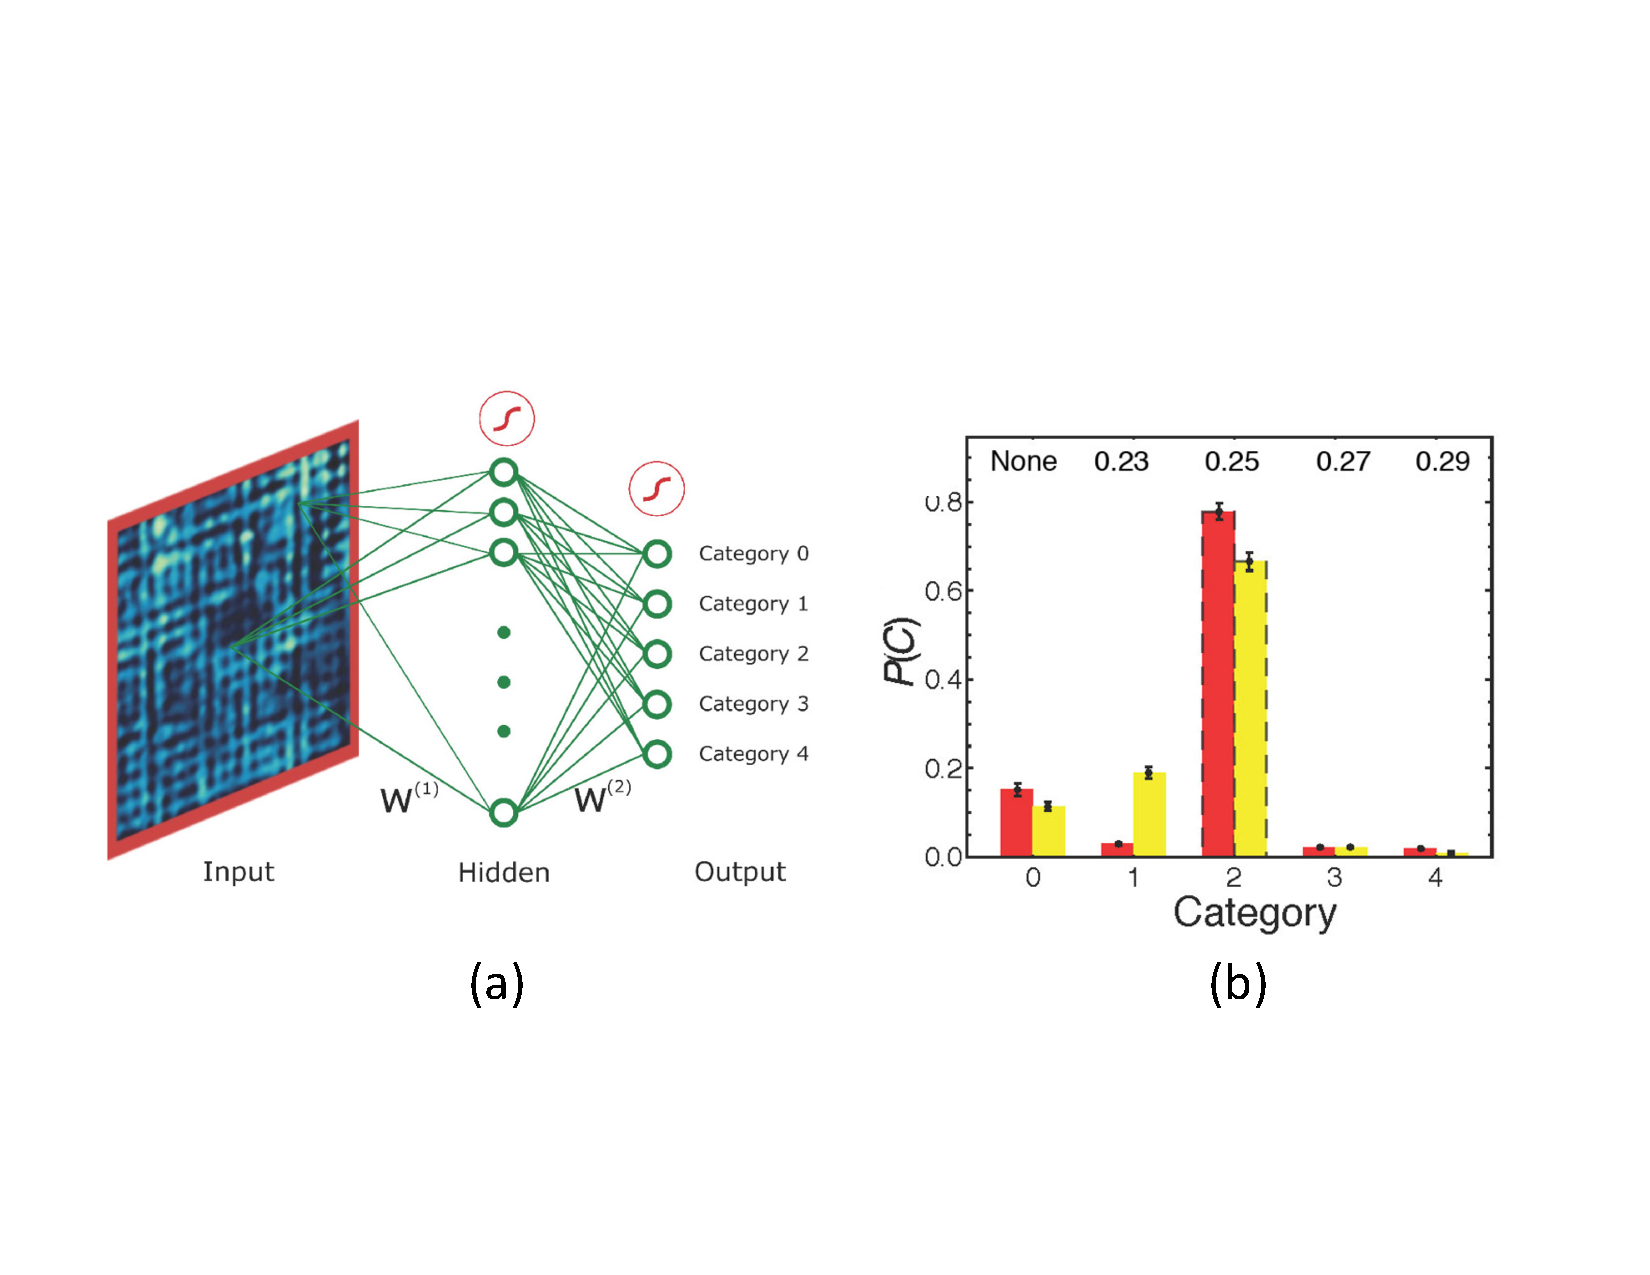
\includegraphics[width=\linewidth]{Manuscript/Figures/STM-results.pdf} 
\caption{(a)The architecture used in Ref.~\cite{Zhang2018}. (b)The classification results for doping XX at energy YY.}
\label{fig:STM-results}
\end{figure}

\subsection{(Roger) Tomography}


\section{Conclusions}
\item Key open issues
	\begin{enumerate}
	\item Interpretability. 
	\item Unsupervised learning on computational and experimental data.
	\item Quantify uncertainty. Unlike many of the industry application where one needs to meet certain qualitative measure (such as realistic images), it is important to ask for quantitative answer when applying ML to physical problems. Thus, to accurately bound (or assess) the uncertainty of the answer like other unbiased computational approaches is desired feature. 
	
	\end{enumerate}
\subsection{Other topics}

%LW: I will shorten these, for now pasted from my notes.
\item Subjects that have been left out, yet are under active development. 

As a new programming paradigm, machine learning naturally changes the computational study of quantum matter, 
    \begin{enumerate}	
    
    \item (Lei) Ab initio calculation:  Material Discoveries: Empirical Potential and Density Functional Theory
	 Accelerating Material discovery via machine learning approaches is an active research frontier. There several layers of opportunities where machine learning can help. 

 %Material database	
 First, it is natural to combine machine learning techniques with materials genome project and high throughput screening of materials and molecules. In its most straightforward application, regression from microscopic composition to the macroscopic properties can be used to bypass laborious ab-initio calculation and experimental search. Finding  appropriate descriptors for materials and molecules sometimes become a key. And such representation learning is exact what deep learning techniques are  designed for. 

 %MD 
 Second, fitting an accurate Empirical Potential with supervised learning already provide a short cut to expensive molecule dynamics simulations~\cite{SchNet, DeepMD}. 

 %DFT 
 Next, within the regime of local density approximation, searching for a good kinetic energy functional can already be extremely useful since it can support orbital free DFT calculations~\cite{Snyder2012, Brockherde2017}. Bypassing Kohn-Sham orbitals (which are auxiliary objects anyway) can greatly accelerate the search of stable material structures. Ultimately, DFT is actually an in principle exact theory, at least for ground state energy and density distribution. However no one knows the universal exchange-correlation functional. Machine Learning modeling of exact density functional has been demonstrated in one dimension~\cite{Li2016} with exact results coming from the density-matrix-renormalization-group calculation in continuous space. For more general realistic cases, besides how to model the density functionals, another problem is how to get accurate training data. 	
  

	\item (Lei) Monte Carlo Approaches.  Monte Carlo is a widely adopted simulation approach in physics and machine learning. A key component of Monte Carlo algorithm is to devise efficient update strategies. 
	
Proposals\cite{Liu2017b}\cite{Xu2017}\cite{Huang2017}
Markov chain Monte Carlo finds wide applications in physics and machine learning. Since the major drawback of MCMC compared to other approximate methods is its efficiency, there is a strong motivation to accelerate MCMC simulations within both physics and machine learning community. In the context of Bayesian statistics, Reference~\cite{Rasmussen2003} trained surrogate functions to speed up hybrid Monte Carlo simulation~\cite{Duane1987}. The surrogate function approximates the potential energy surface of the target problem and provides an easy way to compute derivatives. Recently, there were papers reporting similar ideas for physics problems. Here, the surrogate model can be physical models such as the Ising model~\cite{Liu2017a} or molecular gases~\cite{Huang2017b}, or general probabilistic graphical models such as the restricted Boltzmann machine~\cite{Huang2017a}. For Monte Carlo simulations involving fermion determinants~\cite{Huang2017b, Liu2017fermion} the approach is more profitable since the updates of the original model is much heavier than the surrogate model. However, the actual benefit depends on the particular problem and the surrogate model. A drawback of these surrogate function approaches is that they require training data to start with, which is known as the "cold start" problem in analog to the recommender systems~\cite{Huang2017b}. Using the adaptive approach of~\cite{AdvancedMCMC} one may somewhat alleviate such problem. 
Besides the efficiency boost one can aim at algorithmic innovations in the Monte Carlo updates. Devising novel update strategies which can reduce the auto correlation between samples was considered to be the art MCMC methods. An attempt along this line is Ref.~\cite{Wang2017}, which connected the Swendsen-Wang cluster and the Boltzmann Machines and explored a few new cluster updates. Finally, the NeuralRG \cite{NeuralRG} also provides a fresh approach to perform Monte Carlo updates in the less correlated latent space.

	\item (Lei) Tensor Networks. 
Quantum information perspective offers a significant modern understanding of quantum state of matter. The quantum information measures such as the entanglement entropy quantifies classical resources for modeling quantum states. Exploiting the entanglement pattern of various target states also provides principled guidelines for structural design of various tensor network states. 
Connection to MPS and classes of tensor networks. One approach to assess the expressibility of neural networks is actually to establish a connection to the tensor networks. Since one has developed a large number of theoretical understandings based on the quantum entanglement. \cite{Chen, Gao, Deng} analyzed the expressbility of RBM from the quantum entanglement and computational complexcity perspective. The RBM is more efficient in terms of choosing the describing highly entangled quantum states such as the ones with long range interactions. While the stochastic optimization scheme employed for the RBM is a limiting factor compared to the tensor networks.  
In return, tensor network states also find promising applications in machine learning~ \cite{Stoudenmire}. Tensor network and algorithms provide principled approaches for discriminative and generative tasks with possibly larger expressibility. In fact, the mathematical structure of tensor network stats and quantum mechanics appears naturally when one tries to extend the probabilistic graphical models while still attempts to ensure the positivity of the probability density~\cite{pmlr-v20-bailly11, Zhao-Jaeger}. Moreover, tensor networks are doorways to quantum machine learning~\cite{QMLNature} because the tensor networks are formally equivalent to quantum circuits. By now, tensor networks have caught attentions of practitioners of machine learning~\cite{Levine2017,Cichocki2017}. 
\end{enumerate}
	
	
	
(Roger) Quantum Information: quantum error correction, decoder etc 
(Roger) Reinforcement learning: experimental control 

(Lei: Inverse problem section maybe more relevant than RG to our target audiences. )
(Lei) Inverse problems:  Hamiltonian verification, Analytic Continuation.
Inverse problem are those where the forward solution is straightforward, but the inverse is challenging. This is a ubiquitous situation in physics and engineering. For example, the experimental measurement is a convolution of the physical signal and an kernel function. Typically, the convolution smears out the fine features in the original signal. 
Thus, deconvolution is typically a challenging task, especially with noises on the measured data. One encounters a similar problem when trying to obtain the spectral function from the imaginary-time data obtained in quantum Monte Carlo calculations. In recent years, researchers explored a data driven approach to the inverse problem, where one solves the forward problem many times and trains a machine learning model to identify the inverse mapping. Since the inverse problems are ill-posed without any prior knowledge and assumption, the machine learning approaches provide a way to distill knowledge implicitly contained in the training data. 

(Lei) Renormalization Group, Geometry and Entanglement: It has long been noticed that the neural networks progressively extract more high-level and abstract features in their deep layers, a phenomena resembles the renormalization group. Revealing deep and constructive connection between the two field will on one hand side provide theoretical understanding to deep learning, and on another hand allows one use machine learning machinaries for studying physics. 
	

\end{enumerate}
\section{Glossary}

%We can discuss which ones do we really need
\begin{enumerate}
    \item \textbf{Inductive Bias}: The set of assumptions that the learning algorithm uses to make predictions on new instances which have not been encountered.
    \item \textbf{Back-propagation}: An algorithm to efficiently compute the gradient of the objective function with respect to the neural network parameters. Back-propagation is the computational engine behind the success of training deep neural networks. 
    \item \textbf{Classification and Regression}:
    \item \textbf{Dimensional reduction}:
    \item \textbf{Clustering}:
    \item \textbf{Generative modeling}:
    \item \textbf{Representation Learning}: A set of techniques allow the learning algorithms to identify representations which directly correspond to the discriminative or generative tasks. 
    Learning representation is one of the key notions in modern deep learning research.  
    \item 
\end{enumerate}


\bibliography{AI4CMP-bib}
\end{document}